\documentclass{standalone}
\usepackage{tikz}
\usetikzlibrary{shapes,decorations,shadows}

\usetikzlibrary{calc}


\usetikzlibrary{decorations.text}



\begin{document}


\tikzset{paint/.style={ draw=#1!50!black, fill=#1!50 },
    decorate with/.style=
    {decorate,decoration={shape backgrounds,shape=#1,shape size=2mm}}}




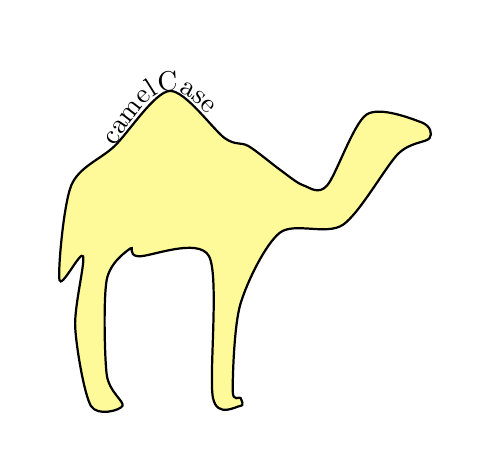
\begin{tikzpicture}

  \path [ultra thick,decorate,decoration={text along path,
            text={camelCase}}] (1.1,3.5) sin (1.8,4.2) cos (2.5,3.6);
  \draw[thick,color=black,fill=yellow!40]
  plot[smooth cycle]
  coordinates{
  (0.55,3) (1.1,3.5) (1.8,4.2) (2.5,3.6) (2.8,3.5) (3.2,3.2) (3.5,3) (3.8,3) (4.3,3.9) (5,3.8) (5.1,3.6) (4.7,3.4) (4,2.5) (3.2,2.4) (2.7,1.5) (2.6,0.4) (2.7,0.3) (2.7,0.2) (2.35,0.3) (2.3,2.1) (1.4,2.1) (1.3,2.2) (1,1.8) (1,0.6) (1.2,0.2) (0.8,0.2) (0.6,1.2) (0.7,2.1) (0.4,1.8) 
  };
  \draw[step=5.5cm,white,very thin] (0,0) grid (5.5,5);     
  
\end{tikzpicture}


\end{document}